\definecolor{boxred}{RGB}{234,99,99}
\definecolor{boxorange}{RGB}{255,242,204}
\definecolor{boxgreen}{RGB}{217,234,211}

\newcommand{\greenbox}{

\begin{tikzpicture}
\draw[line width=0pt, fill=boxgreen]
(0, 0) rectangle (0.3, 0.3);
\end{tikzpicture}}

\newcommand{\orangebox}{

\begin{tikzpicture}
\draw[line width=0pt, fill=boxorange]
(0, 0) rectangle (0.3, 0.3);
\end{tikzpicture}}

\newcommand{\redbox}{

\begin{tikzpicture}
\draw[line width=0pt, fill=boxred]
(0, 0) rectangle (0.3, 0.3);
\end{tikzpicture}}

\chapter{Projektplan}
\section{Änderungsgeschichte}
\begin{tabularx}{\textwidth}{|c|c|X|c|}
  \hline
  \textbf{Datum} & \textbf{Version} & \textbf{Änderung} & \textbf{Autor} \\
  \hline \hline
  26.02.2016 & 1.0 & Erstellen des Projektplans & Martin Stypinski \\
  11.03.2016 & 1.1 & Risiken nach Sprint 1 & Marcel Amsler \\
  26.03.2016 & 1.2 & Risiken nach Sprint 2 & Kirusanth Poopalasingam \\
  12.04.2016 & 1.3 & Risiken nach Sprint 3 & Marcel Amsler \\
  28.04.2016 & 1.4 & Risiken nach Sprint 4 & Kirusanth Poopalasingam \\
  04.06.2016 & 1.5 & Risiken nach Sprint 5 & Martin Stypinski \\
  11.06.2016 & 1.6 & Verantwortlichkeiten dokumentiert & Marcel Amsler \\
  11.06.2016 & 2.0 & Finalisieren des Projektplans & Martin Stypinski \\
  13.06.2016 & 2.0.1 & Qualitätskontrolle und kleinere Korrekturen& Marcel Amsler\\
  \hline
\end{tabularx}

\section{Einleitung}
\subsection{Ziel und Zweck}
Ziel dieser Arbeit ist es, eine Web-Applikation zu entwickeln, die es ermöglicht Drohnenflotten zu verwalten und damit vollautomatisierte Lieferungen auszuführen. Nutzer dieser Applikation können dazu Flugzonen definieren, in denen ein sicherer Flug von Drohnen möglich ist. Kunden hingegen sollen durch eine App die Möglichkeit erhalten, Güter zu bestellen, welche an ihre Position ausgeliefert werden.

\subsection{Lieferumfang}
Der Lieferumfang dieser Arbeit entspricht den Vorgaben der HSR:
\begin{itemize}
	\item{Zu Handen des Betreuers:
	\begin{itemize}
		\item{Dokumentation, sämtliche Dokumente und Sourcen per E-Mail}
	\end{itemize}}
	\item{Poster - Enthält Zusammenfassung der Arbeit}
	\item{Abstract für die Bachelorarbeitsbroschüre}
\end{itemize}
Zusätzlich ist es uns ein Anliegen, dass der Sourcecode und die Erfahrungen über den Zeitraum der Bachelorarbeit hinaus bestehen bleiben. Daher wurde ein GitHub-Repository eingerichtet, dass nach Beendigung der Arbeit sämtlichen Code enthält: \textbf{\url{https://github.com/Project-Helin}}

\subsection{Annahmen und Einschränkungen}
Es kann angenommen werden, dass der Zeitplan im Rahmen der regulären Bachelorarbeit Zeit gültig ist. Es wird dabei berücksichtigt, dass ein Zeithorizont von 17 Wochen zur Verfügung steht und die maximale Arbeitszeit von 360 Stunden pro Person nicht überschritten werden soll.
\section{Projektorganisation}
\subsection{Organisationsstruktur}
\begin{figure}[ht]
%\begin{figure}[H]
	\centering
	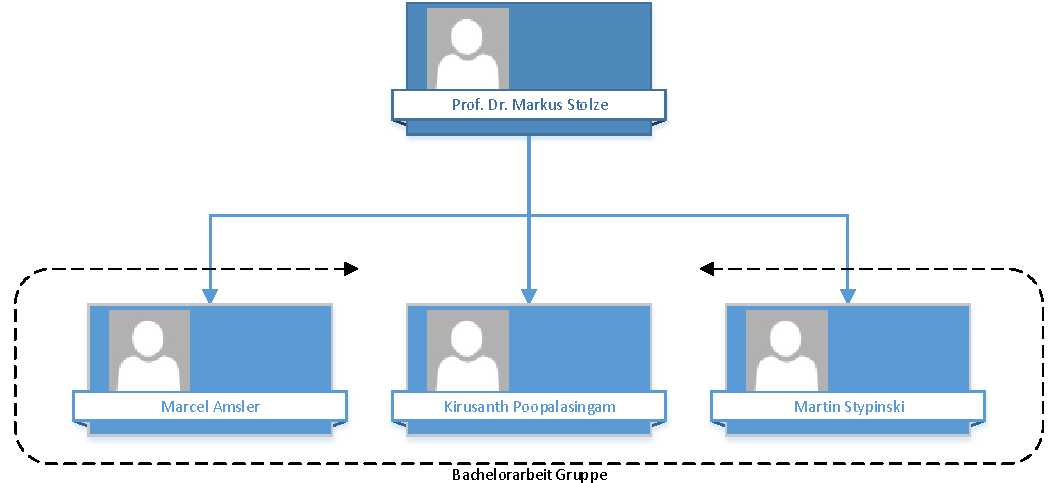
\includegraphics[width=\textwidth]{images/organigram.pdf}
	\caption{Grobübersicht über den Projektplan}
	\label{Risk result}
\end{figure}
\noindent
\begin{tabularx}{\textwidth}{|c|c|c|X|}
  \hline
  \textbf{Name} & & \textbf{E-Mail} & \textbf{Verantwortung} \\
  \hline \hline
  Prof. Dr. Markus Stolze & MST & \url{markus.stolze@hsr.ch} & Betreuer der Arbeit\\
  \hline \hline
  Marcel Amsler & ma &\url{marcel.amsler@hsr.ch} & \\
  \hline
  Kirusanth Poopalasingam & kp & \url{kirusanth.poopalasingam@hsr.ch} & \\
  \hline
  Martin Stypinski & ms & \url{martin.stypinski@hsr.ch} & \\
  \hline
\end{tabularx}
\newpage

\subsection{Verantwortlichkeiten}
Die Verantwortung und eine Unterstützungsfunktion für alle Hauptkomponenten haben wird zu Beginn der Arbeit folgendermassen festgelegt.\\

\begin{tabularx}{\textwidth}{|X|c|c|c|c|}
	\hline
	\textbf{} & \textbf{Server CRUD} & \textbf{Server JavaScript} & \textbf{Onboard-App} & \textbf{Customer App} \\
	\hline 	\hline
	Hauptverantwortung & kp & ms & ma & ma\\
	\hline
	Unterstützung & ms & ma & ms & kp \\
	\hline
\end{tabularx}\\
\newpage


\subsection{Meetings}
In der Regel wird ein Meeting jeweils am Donnerstag um 10.30 abgehalten. In Ausnahmefällen können die Termine von der Planung abweichen.
  \\[1\normalbaselineskip]
\begin{tabularx}{\textwidth}{|c|c|c|X|}
  \hline
  \textbf{SW} & \textbf{Datum} & \textbf{Zeit} & \textbf{Art der Sitzung} \\
  \hline \hline
  1 & 25.02.2016 & 10:00 - 11:00 &  Kick-off Meeting \\
  2 & 03.03.2016 & 15:00 - 16:00 &  Meeting mit Betreuer \\
  3 & 10.03.2016 & 10:30 - 11:30 &  Meeting mit Betreuer \\
  4 & 17.03.2016 & 11:00 - 11:45 &  Meeting mit Betreuer \\
  5 & 24.03.2016 & 10:30 - 11:30 &  Meeting mit Betreuer \\
  6 & 08.04.2016 & 13:30 - 14:30 &  Meeting mit Betreuer \\
  7 & 14.04.2016 & 10:30 - 11:30 &  Meeting mit Betreuer \\
  8 & 21.04.2016 & 10:30 - 11:30 &  Meeting mit Betreuer \\
  9 & 28.04.2016 & 11:00 - 11:45 &  Meeting mit Betreuer \\
  9 & 29.04.2016 & 15:00 - 16:00 &  Zwischenpräsentation bei Prof. Beat Stettler \\
  11 & 11.05.2016 & 18:15 - 19:00 &  Zwischenpräsentation bei Thomas Kälin und Prof. Dr. M. Stolze \\
  11 & 12.05.2016 & 10:30 - 11:30 &  Meeting mit Betreuer \\
  12 & 19.05.2016 & 10:00 - 11:00 &  Meeting mit Betreuer \\
  13 & 26.05.2016 & 10:30 - 11:30 &  Meeting mit Betreuer \\
  14 & 02.06.2016 & 10:30 - 11:30 &  Meeting mit Betreuer \\
  15 & 09.06.2016 & 10:30 - 11:30 &  Meeting mit Betreuer \\
  16 & 13.06.2016 & 10:00 - 11:00 &  Meeting mit Betreuer \\
  \hline
\end{tabularx}
\newpage
\section{Meilensteinplanung}
Grundsätzlich wird während der gesamten Arbeit Agiles-Projektmanagement mit Scrum als Methode eingesetzt. Ein Scrum-Sprint dauert in der Regel 2 Wochen.

\begin{figure}[ht]
%\begin{figure}[H]
	\centering
	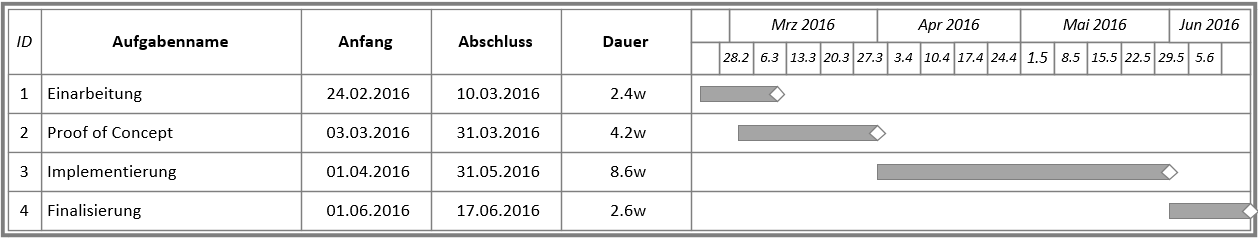
\includegraphics[width=\textwidth]{images/projplan.png}
	\caption{Grobübersicht über den Projektplan}
	\label{Risk result}
\end{figure}

\begin{itemize}
	\item{\textbf{Ende Einarbeitung: (MS-1)} 
		\begin{itemize}
			\item{\textbf{Datum:} 11.03.2016}
			\item{\textbf{Ziel:} Entwicklungsumgebung und Prozesse stehen}
			\item{\textbf{Erfüllungskriterium:} Sämtliche prozessbegleitenden Massnahmen sind lauffähig.\\ Projektmanagement-Tool, IDEs, CI}
		\end{itemize}
	}
	
	\item{\textbf{Ende Proof of Concept: (MS-2)} 
		\begin{itemize}
			\item{\textbf{Datum:} 25.03.2016}
			\item{\textbf{Ziel:} Die Machbarkeit ist bewiesen}
			\item{\textbf{Erfüllungskriterium:} Prototyp ist lauffähig, zeigt Machbarkeit und allfällige Einschränkungen.}
		\end{itemize}
	}
	
	\item{\textbf{Ende Implementierung: (MS-3)} 
		\begin{itemize}
			\item{\textbf{Datum:} 03.06.2016}
			\item{\textbf{Ziel:} Code Freeze}
			\item{\textbf{Erfüllungskriterium:} Alle zwingenden funktionalen und nicht-funktionalen Anforderungen sind erfüllt.}
		\end{itemize}
	}	
	\item{\textbf{Abgabe: (MS-4)} 
			\begin{itemize}
				\item{\textbf{Datum:} 17.06.2016}
				\item{\textbf{Ziel:} Abgabe der Arbeit}
				\item{\textbf{Erfüllungskriterium:} Alle im Lieferumfang geforderten Dokumente sind fertiggestellt}
			\end{itemize}
	}
	
\end{itemize}

\newpage


\begin{landscape}
\section{Risikomanagement}
\subsection{Risiken}
\LTXtable{0.75\paperheight}{risk.tex}
\end{landscape}
\subsection{Umgang mit Risiken}
Die Risiken wurden in einer Risiko Matrix aufgegliedert um besser zu verstehen, welche Risiken eine grosse Bedrohung darstellen.

\begin{figure}[ht]
%\begin{figure}[H]
	\centering
	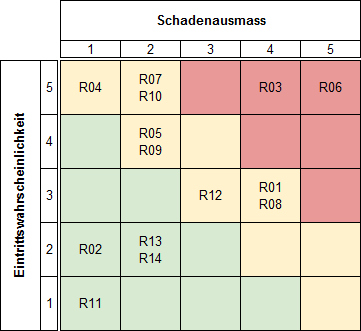
\includegraphics[scale=0.7]{images/risk_result.png}
	\caption{Risiko Matrix}
	\label{Risk result}
\end{figure}

Als Konsequenz der Matrix kann folgende Aufteilung getroffen werden:
\begin{itemize}
	\item{\textbf{Risiko hoch:} R03, R06}
	\item{\textbf{Risiko mittel:} R01, R04, R05, R07, R08, R09, R10, R12 }
	\item{\textbf{Risiko klein:} R02, R11, R13, R14}
\end{itemize}

\subsection{Massnahmen}
Für die Risiken der Kategorie mittel und hoch wurden folgende Massnahmen festgelegt:
\begin{itemize}
	\item{\textbf{R03 - Internet auf Mobilgerät:} \\
	\textbf{Massnahmen:} Es muss sichergestellt werden, dass die Drohne nicht auf eine permanente Serververbindung angewiesen ist. Monitor und Datenlogging dürfen Unterbrechungen aufweisen. Die Mission darf aber zu keinem Zeitpunkt gefährdet werden, die Drohne muss selbstständig ihre Aufgabe erfüllen können und danach wieder zurückkehren.}
	
	\item{\textbf{R06 - Absturz und Schäden:} \\
	\textbf{Massnahmen:} Bei der Wahl der Drohne wurde auf die Verfügbarkeit der Ersatzteile geachtet, sofern dies möglich war. }

	\item{\textbf{R01 - Messaging auf Mobilgerät:} \\
	\textbf{Massnahmen:} Bei der Evaluierung der Komponenten wird ein Message-Broker gewählt, der auf einem Android Betriebssystem lauffähig ist. Dies wird in einem Proof of Concept überprüft.}
	
	\item{\textbf{R04 - Infrastruktur Probleme:} \\
	\textbf{Massnahmen:} Aufgrund von Erfahrungen aus früheren Projekten, wird auf die Serverinfrastruktur der HSR verzichtet, dies garantiert eine volle Kontrolle über den Server. Es muss jedoch berücksichtig werden, dass der administrative Aufwand höher ist und somit mehr Zeit in Anspruch nehmen wird.}
	
	\item{\textbf{R05 - Kapazität der Drohne:} \\
	\textbf{Massnahmen:} Es werden Güter verwendet, deren Gewicht von der Drohne transportiert werden kann.}	
	
	\item{\textbf{R07 - Positionsungenauigkeit:} \\
	\textbf{Massnahmen:} Bei Flugkorridoren und Landepunkten wird genügend Sicherheitsmarge eingerechnet um die Ungenauigkeit zu relativieren.}
	
	\item{\textbf{R08 - Ardupilot Handhabung:} \\
	\textbf{Massnahmen:}  Im Proof of Concept wird überprüft, wann und wie Updates gemacht werden können. Falls Updates während des Flugs nicht möglich sind, wird von Anfang an die gesamte Route an Ardupilot übertragen.}
	
	\item{\textbf{R09 - Ardupilot API:} \\
	\textbf{Massnahmen:} Früh in einem Proof of Concept die Möglichkeiten und Grenzen des APIs nachvollziehen.}
	
	\item{\textbf{R10 - Entwicklungsprozesse:} \\
	\textbf{Massnahmen:} Es wird während des Proof of Concepts versucht einen Simulator zu verwenden, um Zeit zu sparen. Gegebenenfalls Arbeitsplatz im Freien, um Zeit während des Deployments auf die Drohne zu sparen.}
	
	\item{\textbf{R12 - Ablademanagement:} \\
	\textbf{Massnahmen:} Prüfung einer Abwurfmöglichkeit. Gegebenenfalls Benutzer mit GUI auf Mobile begleiten um einen sicheren und unfallfreien Abladevorgang zu garantieren.}
\end{itemize}

\newpage
\section{Qualitätsmassnahmen}	
\subsection{Dokumentation}
Die Dokumentation wird vollständig in Latex geschrieben und befindet sich zu jedem Zeitpunkt auf dem Project-Helin GitHub-Repository: \url{https://github.com/Project-Helin}. Alle grösseren Änderungen werden immer von einem anderen Teammitglied gelesen und überprüft.

\subsection{Projektmanagement}
Für das Projektmanagement wird Jira von Atlassian verwendet. Als Projektmanagement Methode wird Scrum verwendet.

\subsection{Entwicklung}
Die Qualität der Entwicklung wird durch folgende Massnahmen sichergestellt:
\begin{itemize}
	\item{\textbf{Code Review:} Bei kritischen Komponenten werden Code Reviews durchgeführt.}
	
	\item{\textbf{Feature Review:} Bei allen Features bzw. umgesetzten User-Stories führt ein anderes Teammitglied eine Qualitätskontrolle durch. Diese kontrolliert hauptsächlich die Erfüllung der Acceptance-Criterias.}
	
	\item{\textbf{Testing:} Das gesamte Projekt wird in Java entwickelt. Als Unit-Test Framework wird JUnit 4 verwendet.}
	
	\item{\textbf{Versionierung:} Der gesamte Quellcode wird mit Hilfe von GitHub versioniert.}
	
	\item{\textbf{Deployment:} Die Serverkomponenten werden mithilfe eines Build Systems deployt. Die Komponenten auf den Mobiltelefonen werden manuell deployt. Jedoch wird auf dem Build-System für alle Komponenten die Ausführung von Unit-Tests garantiert.}
	
\end{itemize}

\newpage
